\documentclass{beamer}
\usepackage{amsmath,amsbsy,amsopn,amstext,amsfonts,amssymb}
\usepackage{isomath}
\usepackage{ulem}
%\linespread{1.6}  % double spaces lines
\usepackage{graphicx}
\usepackage{subfigure}
\usepackage{color}
\usepackage{optidef}  % define optimization problems
\usepackage{multicol}  % multiple columns
\usepackage{listings} % for python code
\usepackage{mathrsfs}

\usepackage{polynom}
\newcommand{\adj}{\mathrm{adj}}
\newcommand{\constrainedmin}[3]{
		\begin{mini*}|s|
		{#2}{#1}{}{}
		\addConstraint{#3}
		\end{mini*}
}

\newcommand{\rwbcomment}[1]{{\color{blue}RWB:#1}}
\newcommand{\defeq}{\stackrel{\triangle}{=}}
\newcommand{\abs}[1]{\left|#1\right|}
\newcommand{\norm}[1]{\left\|#1\right\|}
\newcommand{\iprod}[1]{\left<#1\right>}
\newcommand{\ellbf}{\boldsymbol{\ell}}
\newcommand{\nubf}{\boldsymbol{\nu}}
\newcommand{\mubf}{\boldsymbol{\mu}}
\newcommand{\abf}{\mathbf{a}}
\newcommand{\bbf}{\mathbf{b}}
\newcommand{\cbf}{\mathbf{c}}
\newcommand{\dbf}{\mathbf{d}}
\newcommand{\ebf}{\mathbf{e}}
\newcommand{\fbf}{\mathbf{f}}
\newcommand{\gbf}{\mathbf{g}}
\newcommand{\hbf}{\mathbf{h}}
\newcommand{\ibf}{\mathbf{i}}
\newcommand{\jbf}{\mathbf{j}}
\newcommand{\kbf}{\mathbf{k}}
\newcommand{\lbf}{\mathbf{l}}
\newcommand{\mbf}{\mathbf{m}}
\newcommand{\nbf}{\mathbf{n}}
\newcommand{\obf}{\mathbf{o}}
\newcommand{\pbf}{\mathbf{p}}
\newcommand{\qbf}{\mathbf{q}}
\newcommand{\rbf}{\mathbf{r}}
\newcommand{\sbf}{\mathbf{s}}
\newcommand{\tbf}{\mathbf{t}}
\newcommand{\ubf}{\mathbf{u}}
\newcommand{\vbf}{\mathbf{v}}
\newcommand{\wbf}{\mathbf{w}}
\newcommand{\xbf}{\mathbf{x}}
\newcommand{\ybf}{\mathbf{y}}
\newcommand{\zbf}{\mathbf{z}}
\newcommand{\Jbf}{\mathbf{J}}
\newcommand{\Acal}{\mathcal{A}}
\newcommand{\Bcal}{\mathcal{B}}
\newcommand{\Lcal}{\mathcal{L}}
\newcommand{\Ncal}{\mathcal{N}}
\newcommand{\Rcal}{\mathcal{R}}
\definecolor{darkolivegreen}{rgb}{0.33, 0.42, 0.18}

\makeatletter
\newenvironment<>{proofstart}[1][\proofname]{%
    \par
    \def\insertproofname{#1\@addpunct{.}}%
    \usebeamertemplate{proof begin}#2}
  {\usebeamertemplate{proof end}}
\newenvironment<>{proofcont}{%
  \setbeamertemplate{proof begin}{\begin{block}{}}
    \par
    \usebeamertemplate{proof begin}}
  {\usebeamertemplate{proof end}}
\newenvironment<>{proofend}{%
    \par
    \pushQED{\qed}
    \setbeamertemplate{proof begin}{\begin{block}{}}
    \usebeamertemplate{proof begin}}
  {\popQED\usebeamertemplate{proof end}}
\makeatother

\title{ECEn 671: Mathematics of Signals and Systems}
\author{Randal W. Beard}
\institute{Brigham Young University}
\date{\today}

\begin{document}

%-------------------------------
\begin{frame}
	\titlepage
\end{frame}


%%%%%%%%%%%%%%%%%%%%%%%%%%%%%%%%%%%%%%%%%%%%%%%%%%%%%%%%%%%%%%%%%
\section{Recursive Least Squares Filtering}
\frame{\sectionpage}

%----------------------------------
\begin{frame}\frametitle{Least Squares Filtering Problem}
	\begin{figure}
		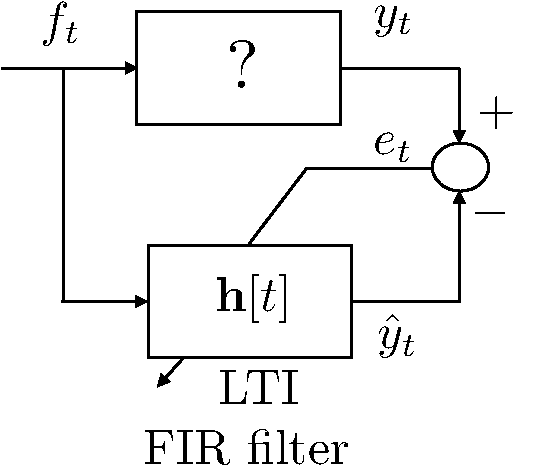
\includegraphics[width=0.5\textwidth]{figures/chap4_rls}	
	\end{figure}
	
	{\bf Problem Statement:}  Given the input data $f_t$ and $y_t$, find the FIR filter coefficients $\hbf[t]$ that minimize the running least squared error $e_t$.
	
\end{frame}



%----------------------------------
\begin{frame}\frametitle{Least Squares Filtering Problem}
	\begin{definition}[Least Squares Filtering Problem]
		Given the filter
		\[ \hat{y}_t = \sum_{i=1}^m h_i f_{t-i} \]
		where the inputs $f_t$ are known and we measure the actual outputs $y_t$, 
		find the coefficients $h_i$ such that the mean squared error 
		\[
		E = \sum_{i=1}^m \left( y_i-\hat{y}_i \right)^2
		\]
		is minimized.
	\end{definition}
\end{frame}

%----------------------------------
\begin{frame}\frametitle{Batch Least Squares Filtering}
	If we assume $f_t = 0, t \leq 0$ we get
	{\footnotesize
	\[
		\begin{pmatrix}
	 		y_1\\
 	   		y_2\\
 	   		\vdots\\
 	   		y_N
 	   	\end{pmatrix}
 	   	=
 	   	\begin{pmatrix}
   	  		f_1 & 0 & \cdots & \cdots & 0\\
  	  		f_2 & f_1 & 0 & \cdots & 0\\
    		\vdots & & & \ddots\\
    		f_m & f_{m-1} & \cdots & \cdots & f_1 \\
    		f_{m+1} & f_m & f_{m-1} & \cdots & f_2 \\
    		\vdots & & & \ddots \\
    		f_N & f_{N-1} & \cdots & \cdots & f_{N-m+1}
    	\end{pmatrix}
    	\begin{pmatrix}
    		h_1 \\
    		h_2 \\
    		\vdots\\
    		h_m
    	\end{pmatrix}
	\]
	}
\end{frame}

%----------------------------------
\begin{frame}\frametitle{Batch Least Squares Filtering, cont.}
	Define
	\begin{align*}
		\qbf_i &= \begin{pmatrix} f_i & f_{i-1} & \dots f_{i-m+1} \end{pmatrix}^H \\
		\ybf_N &= \begin{pmatrix} \bar{y}_1 & \bar{y}_2 & \dots \bar{y}_N \end{pmatrix}^H \\
		\hbf[N] &= \begin{pmatrix} \bar{h}_1[N] & \bar{h}_2[N] & \dots \bar{h}_m[N] \end{pmatrix}^H \\
		A_N &= \begin{pmatrix} \qbf^H_1 \\ \vdots \\ \qbf^H_m \end{pmatrix},
	\end{align*}
	then the least squares problem reduces to
	\[ 
		\ebf_N = \ybf_N - \underbrace{A_N \hbf[N]}_{\hat{\ybf}_N}
	\] 
	where $\ebf_N$ is the error to be minimized.  From the projection theorem, $\norm{\ebf}_2$ is minimized when
	\[
		\underset{m\times 1}{\hbf[N]} = (\underset{m \times N}{A^H_N} \underset{N \times m}{A_N)}^{-1}\underset{m\times N}{A^H_N}\underset{N\times 1}{\ybf_N}. 
	\]
\end{frame}

%----------------------------------
\begin{frame}\frametitle{Batch Least Squares Filtering}
	\begin{itemize}
		\item Note that the size of $y_N$ and $A_N$ grow linearly with time $N$.  
		\item Therefore, each time step requires more computation than the last step.  This is obviously problematic as $N\to\infty$.  
		\item For some $N$, batch least squares is no longer a real-time algorithm.
		\item Note that at time $N+1$ the data include new samples, but includes all of the data available at time $N$.
	\end{itemize}
	
	\vspace{1cm}
	
	{\color{red} ???  Is is possible to design an algorithm with fixed computational cost at each time step, that produces the same least squares solution?}
\end{frame}

%----------------------------------
\begin{frame}\frametitle{Recursive Least Squares Filtering}
	Define
	\begin{align*}
		\qbf_t &= \begin{pmatrix} f_i & f_{i-1} & \dots f_{i-m+1} \end{pmatrix}^H \\
		\ybf_t &= \begin{pmatrix} \bar{y}_1 & \bar{y}_2 & \dots \bar{y}_t \end{pmatrix}^H \\
		\hbf[t] &= \begin{pmatrix} \bar{h}_1[t] & \bar{h}_2[t] & \dots \bar{h}_m[t] \end{pmatrix}^H \\
		A_t &= \begin{pmatrix} \qbf^H_1 \\ \vdots \\ \qbf^H_t\end{pmatrix}.
	\end{align*}
	Then at time $t$ we have $\ebf_t = \ybf_t - A_t \hbf[t]$.  From the projection theorem, the error is minimized when
	\[
		\hbf[t] = (A^H_t A_t)^{-1} A_t^H \ybf_t.
	\]
\end{frame}

%----------------------------------
\begin{frame}\frametitle{Recursive Least Squares Filtering, cont.}
	Let 
	\begin{align*}
		R_{t-1} &\defeq A^H_{t-1} A_{t-1} 
		     = \begin{pmatrix}\qbf_1 & \cdots & \qbf_{t-1}\end{pmatrix} \begin{pmatrix} \qbf^H_1 \\ \vdots \\ \qbf^H_{t-1} \end{pmatrix} \\
		    &= \sum_{i=1}^{t-1} \qbf_i \qbf^H_i
	\end{align*}
	be the associated Grammian when there are $t-1$ samples.  
	
	\vfill
	
	Suppose that we receive new data $q_t$ and $y_t$ at time $t$.
	
	\vfill
	
	Then 
	\begin{align*}
		R_t &= \sum_{i=1}^{t} \qbf_i \qbf^H_i \\
		    &= \sum_{i=1}^{t-1} \qbf_i \qbf^H_i  + \qbf_t \qbf_t^H \\
		    &= R_{t-1} + \qbf_t \qbf_t^H.
	\end{align*}
\end{frame}

%----------------------------------
\begin{frame}\frametitle{Recursive Least Squares Filtering, cont.}
	In the solution $\hbf_t = (A_t^H A_t)^{-1} A_t^H \ybf_t$, we need $R_t^{-1} \defeq (A_t^H A_t)^{-1}$.
	
	Note that 
		\[R_t^{-1} = (\underbrace{R_{t-1}}_{A} + \underbrace{q_t}_{X}\underbrace{}_{R=1}\underbrace{q_t^H}_{Y})^{-1}\] 
	and recall the matrix inversion lemma:
		\[ (A + XRY)^{-1} = A^{-1} - A^{-1}X(R^{-1}+YA^{-1}X)^{-1}YA^{-1} \]
	Therefore
		\[R_t^{-1} = R_{t-1}^{-1} - R^{-1}_{t-1} \qbf_t(1 + \qbf_t^H R^{-1}_{t-1} \qbf_t)^{-1}\qbf_t^H R^{-1}_{t-1}.\]
\end{frame}

%----------------------------------
\begin{frame}\frametitle{Recursive Least Squares Filtering, cont.}

	Defining $P_t = R_t^{-1}$ gives
		\[
		P_t = P_{t-1} - \frac{P_{t-1} \qbf_t \qbf_t^H P_{t-1}}{1 + \qbf_t^H P_{t-1} \qbf_t}.
		\]
	Define the (Kalman) gain as
		\[ 
		\kbf_t = \frac{P_{t-1} \qbf_t}{1 + \qbf_t^H P_{t-1} \qbf_t}
		\]
	Then
	\[ 
	P_t = P_{t-1} - \kbf_t \qbf_t^H P_{t-1}. 
	\]
	Note that we have found a fixed computational scheme to update
	\[
	P_t = (A_t^H A_t)^{-1} 
	\]
	using old data $P_{t-1}$ and new data $\qbf_t$.
\end{frame}


%----------------------------------
\begin{frame}\frametitle{Recursive Least Squares Filtering, cont.}
		In the solution $\hbf[t] = (A_t^H A_t)^{-1} A_t^H \ybf_t$, we have found a clever way to update $P_t=(A_t^H A_t)^{-1}$ recursively.  Define
		\[
		\zbf_t \defeq A_t^H \ybf_t.
		\]
		We need a recursive update for $\zbf_t$.
		
		Toward that end note that
		\begin{align*}
			\zbf_t &= A_t^H \ybf_t \\
			 	&= \sum_{i=1}^t \qbf_i y_i \\
			 	&= \sum_{i=1}^{t-1} \qbf_i y_i + \qbf_t y_t \\
				&= \zbf_{t-1} + \qbf_t y_t
		\end{align*}
\end{frame}

%----------------------------------
\begin{frame}\frametitle{Recursive Least Squares Filtering, cont.}
	Therefore
	\begin{align*}
		\hbf_t	&= (A_t^H A_t)^{-1} A_t^H \ybf_t \\
				&= P_t \zbf_t \\
				&= (P_{t-1} - \kbf_t \qbf_t^H P_{t-1})(\zbf_{t-1} + \qbf_t y_t)\\
				&= P_{t-1} \zbf_{t-1} - \kbf_t \qbf_t^H P_{t-1} \zbf_{t-1} + P_{t-1} \qbf_t y_t - \kbf_t \qbf_t^H P_{t-1} \qbf_t y_t\\
				&= \hbf_{t-1} - \kbf_t \qbf_t^H \hbf_{t-1} + \underbrace{\left( P_{t-1}-\kbf_t \qbf_t^H P_{t-1} \right)}_{P_t} \qbf_t y_t \\
				&= \hbf_{t-1} + \kbf_t(y_t - \qbf_t^H \hbf_{t-1}) \\
		\implies \hbf_t &= \hbf_{t-1} + \kbf_t(y_t - \hat{y}),
	\end{align*}
	where we have used the fact that $P_t q_t = \kbf_t$.

	Note that $\hat{y}_t = \qbf_t^H \hbf_{t-1}$ is the predicted output, and $e_t=y_t-\hat{y}_t$ is the quantity that is being minimized.
\end{frame}

%----------------------------------
\begin{frame}\frametitle{Summary: Recursive Least Squares Filtering}
	At time $t=0$ initialize algorithm with
	\begin{align*}
		P_0 &= \alpha I, \text{~where $\alpha>0$ is a large number} \\
		\hbf_0 &= 0.
	\end{align*}
	At time $t$, get $y_t$, $f_t$, and compute $\qbf_t$ from $f_t$.  Update the least squares estimate using  
	\begin{align*}
  		\kbf_t &= \frac{P_{t-1} \qbf_t}{1 + \qbf_t^H P_{t-1} \qbf_t} \\
  		P_t &= P_{t-1} - \kbf_t \qbf_t^H P_{t-1} \\
  		\hbf_t &= \hbf_{t - 1} + \kbf_t (y_t - \qbf_t^H \hbf_{t-1}).
	\end{align*}
This is equivalent to a discrete time Kalman filter with stationary dynamics.
	
\end{frame}




\end{document}